\documentclass[sigconf]{acmart}
\settopmatter{printacmref=false} % Removes citation information below abstract
\renewcommand\footnotetextcopyrightpermission[1]{} % removes footnote with conference information in first column
\pagestyle{plain} % removes running headers
\usepackage{booktabs} % For formal tables
\usepackage{float}
\usepackage[]{algorithm2e}
\usepackage{multirow}


% Copyright
\setcopyright{none}
%\setcopyright{acmcopyright}
%\setcopyright{acmlicensed}
%\setcopyright{rightsretained}
%\setcopyright{usgov}
%\setcopyright{usgovmixed}
%\setcopyright{cagov}
%\setcopyright{cagovmixed}


\begin{document}
\title{Ranking and Prediction of Amazon Fine Food based on Costumer's rating and review}

\author{Ng Wing Hin}
\affiliation{%
  \institution{Chinese University of Hong Kong}
}
\email{1155106860@link.cuhk.edu.hk}

\author{Lei Wen Fen}
\affiliation{%
  \institution{Chinese University of Hong Kong}
}
\email{1155002533@link.cuhk.edu.hk}

\author{Cheng Tin Chu}
\affiliation{%
  \institution{Chinese University of Hong Kong}
}
\email{1155106571@link.cuhk.edu.hk}

\author{Chan Hei Nam}
\affiliation{%
  \institution{Chinese University of Hong Kong}
}
\email{1155103957@link.cuhk.edu.hk}

\graphicspath{ {images/} }

\begin{abstract}
This project uitilize the Amazon Fine Food data set from Kaggle to implement a system that can predict rating based on user's comment. We will be using varies algorithms from big data to anaylsis the data set. In the end of this project, we are expected to observe the relationship between user's comments and rating. By comparing the result to test data we can do prediction of rating based on the similarity of the comments. Moreover, we will come up with the most and least popularity of products based on rating.
\end{abstract}
\keywords{Big Data System, Document anaylsis, Prediction Model}
\maketitle

\section{Introduction}
Currently, we are all living in a social system under capitalism. Every enterprise is competing with each other with their own products, services and even user experience. With the rapid growth of the internet in recent year, user experience can be further improved via processing huge data on costumer's review and rating. The Large internet-based retailer, like Amazon, have an enormous number of products but obviously, not all of them are popular. Therefore, processing costumer's review and rating of a product is vital for improving user experience thus increasing profit.

In order to determine the popularity of a product, an explicit way is to process costumer's review and rating. Nonetheless, the number of responses on a product would not always be sufficiently large enough for reference. In the Amazon Fine Food Reviews, there are user's scores and reviews on different products and our goal is to investigate the popularity of products by these two factors. This will benefit online retailer to promote further actions to enhance user experience and yield more revenue. Moreover, the system would be able to do predication of rating of the product based on the comment.


\section{Problem Setting}
Given a dataset of all review records \(\mathfrak{D}\), we first remove some stopwords that the result maintain the same positivity or negativity as the original comment. We then apply k-shingles on comments \(\mathfrak{C}\) for each rating values and use MapReduce to count the frequency of each shingle and respective rating. Using the result, we want to train our system using regression. Finally, the system would be able to predict the score based on given comments.

\subsection{Basic Statistic of the dataset}
Before we explain the structure of our system, we will be looking at basic statistic of the data set we will be using. 
\begin{table}[H]
  \caption{Basic Statistic of the rating}
  \label{tab:commands}
  \begin{tabular}{ll}
  	\toprule
    & Score \\ 
    \midrule
    Mean & 4.18 \\
    Std & 1.31 \\ 
    Min & 1 \\
    First Quartile & 4 \\
    Median & 5 \\
    Third Quartile & 5 \\
    Max & 5 \\ 
    \bottomrule
  \end{tabular}
\end{table}

\begin{table}[H]
  \caption{Basic Statistic of the rating}
  \label{tab:commands}
\begin{tabular}{lll}
	\hline
	    					& Rating 	& Word(Processed)\\
	\hline
	Mean					& 4.18 		& 255\\
%	Standard Deivation	& 1.31		& \\
	Minimum       		& 1 			& 7\\
	Maximum       		& 5 			& 14425\\
%	First Quartile 		& 4 			& 				& \\
%	Median 				& 4 			& 				& \\
%	Third Quartile 		& 5 			& 				& \\
	\hline
\end{tabular}
\end{table}

\begin{table*}
  \caption{Original Data}
  \label{tab:commands}
  \begin{tabular}{l}
    \toprule
    Id , ProductId, UserId, ProfileName, HelpfullnessNumerator, HelpfullnessDenominator, Score, Time, Summary, Text\\
    \midrule
    1,B001E4KFG0,A3SGXH7AUHU8GW,delmartian,1,1,5,1303862400,Good Quality Dog Food,I have bought... \\
    2,B00813GRG4,A1D87F6ZCVE5NK,dll pa,0,0,1,1346976000,Not as Advertised,"Product arrived labeled...\\
    3,B000LQOCH0,ABXLMWJIXXAIN,"Natalia Corres ""Natalia Corres""",1,1,4,1219017600,"""Delight"" says it all","This is a confection...\\
    4,B000UA0QIQ,A395BORC6FGVXV,Karl,3,3,2,1307923200,Cough Medicine,If you are looking... \\
    \bottomrule
  \end{tabular}
\end{table*}

\begin{table*}
  \caption{Part of Result Dataset}
  \label{tab:commands}
  \begin{tabular}{ll}
    \toprule
    Score & Text\\
    \midrule
	5 & bought vitality canned dog food products good quality product looks like stew processed meat smells ... \\ 
	1 & product arrived labeled jumbo salted peanutsthe peanuts actually small sized unsalted not sure error  ... \\ 
	4 & confection centuriesit light pillowy citrus gelatin nutsin case filberts cut tiny squares liberally coated powdered  ...\\ 
	2 & looking secret ingredient robitussin believe iti got addition root beer extract ordered good cherry sodathe  ... \\ 
	\bottomrule
  \end{tabular}
\end{table*}

\section{System Structure}
In this project, we will be using python to code the system that perform processing on the data set. There are three stages in the whole system, we will be explaining the idea and coding in the following subsections. Based on the result generated by each stage we can do prediction of rating based on the give comment.

\subsection{Methodology}
The prediction was based on k-shingle approach. The main steps were first to extract sample shingles from training set and then to predict the score by matching them. Shingle length of 1 to 5 were focused and this was considered according the average size of review comments. The further shingle length was not useful due to extremely low repeat rate.

Two approaches for the default score were compared: the middle score of score range and the average score of training set. Default score was required to assign the score if no shingle was matched from the sample shingle set.

Two prediction methods were implemented: k-shingle predicted score and Regression Method. The first method was calculated by matching shingles. However, each k-shingle prediction only focused on its own k-shingle information. We would like to explore an approach to gather all the information and test whether a more accurate result could be achieved.

A straight forward idea would be taking an average from the five k-shingle predicted scores; nevertheless, this deemed all the shingle scores were equally important. And if there were matched 5-shingles, the 5-shingle predicted score should be more representable and with higher weight.

Therefore, the Regression Method was introduced as an objective approach to investigate the linkage among the five k-shingle predicted scores. In this project, this method was executed by using linear regression.

Figure 1 is the flowchart of the system, white parallegram is data file while blue square is the program we code.

\begin{figure}
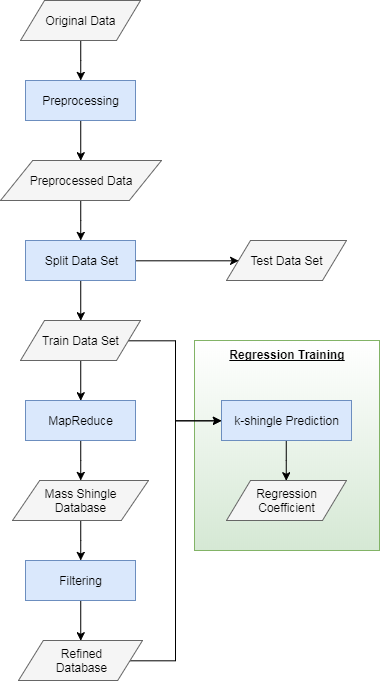
\includegraphics[height=4.5in, width=2.8in]{flowchart}
\caption{Flowchart of the system}
\end{figure}

\subsection{Stage 1 - Data Preprocessing}
In this subsection, we will be explaining the idea behind stage one, pre-processing. As only small portion of the given data are useful in this project, we need to do pre-processing before doing other applications.

We will be looking at the algorithm for data preprocessing: 

\begin{algorithm}
\caption{Preprocessing}
\DontPrintSemicolon
\KwData{Reviews.csv}
\KwResult{Preprocessed.csv}

 \While{There exists next row inside Reviews.csv}
 {
 	Extract \textbf{Rating} and \textbf{Text}\;
 	Lower \textbf{Text} and remove \emph{some} stopwords and punctuation\;
 	Returning line with format \(Rating, word_{1}, word_{2}, ...\)\;
 }
\end{algorithm}


The original data file is in format of \(.csv\), each column is separated by a comma and each row is separated by a linebreak. Each row have the format : \{Id , ProductId, UserId, ProfileName, HelpfullnessNumerator, HelpfullnessDenominator, Score, Time, Summary, Text\}. As mentioned before, the only important parts are Score and Text. Thus, the resulting data have format : \{Score, Text\}. 

During the pre-process, we will extract rating column, summary column and comment column of each review record. Moreover, we will remove all punctuations and selected stopwords from comment part and left with only meaningful words. The stopwords list from [2] was taken as reference, but some stopwords were preserved because it affected the real meaning of the comment. For example, "Good" and "Not Good". If we remove stopword "Not", the meaning of the comment is completely reversed. Therefore, "contrast" stopwords were remained, such as, "but", "however, "not" and "yet". "Emphasis" stopwords were also kept, for example, "indeed", "very", "must", "never", "only". The following illustrated how a sentence was transformed:\\

\begin{tabular}{l|l}
  %\toprule
	
  \midrule
  	\multirow{2}{*} {Original sentence} &
  	This is a very very good product, but \\
  	& there is room for improvement.\\
  	\hline
	\multirow{2}{*} {Preprocessed} &
	very very good product but room \\
	& improvement \\
  \bottomrule
\end{tabular}\\


As the length of comment was in paragraph size, the above wordings were vital for sentiment analysis. Especially, the project attempted to predict scores from 1 to 5, instead of positive, neutral or negative, every words matters. For instance, "very good", the "emphasis" word "very" may helped to distinguish from "good" and hence, the former may be score of 5; while the latter may be 4.

After the preprocessing is finished, we will split 70\% of the dataset as training set and 30\% as testing set.

Let us observe part of the original data and the result from pre-processing before we explain how we do pre-processing in Table 3 and Table 4.




\subsection{Stage 2 - Construction of Shingle-Score Database}
At first, the mass shingle-score database was constructed by MapReduce among the training set. The mapper generated 1-shingles to 5-shingles for each review. The key is \(\{Score,\mbox{ } Shingle\mbox{ } Length,\mbox{ } Shingle\}\) and the value is "1". During the shuffle and sorting stage, same key value's tuples were gathered and the reducer summed all the 1's to count the frequency. In order to confine the data, shingles with count of 1 were excluded.
This not only reduced the size of output, but also filtered out unnecessary shingles. For example, a shingle that appeared only once was not meaningful for prediction and it required a considerable size of storage to store all of them.
In general, a frequency threshold could be set for this step.

Here is the algorithm for mapper and reducer:
\begin{algorithm}
\DontPrintSemicolon
\KwData{Preprocessed.csv}
\KwResult{Tuple}
\caption{Mapper}
	\While{There exists next row inside Preprocessed.csv}
	{
		\For{$k \leftarrow 1$ \KwTo $5$}
		{
			\label{forins}
			Find all k-shingles\;
			\For{Each shingle found}
			{
				Return \(<<\mbox{rating, k, shingle}>, 1>\);
			}
 		}
	}
\end{algorithm}

\begin{algorithm}
\DontPrintSemicolon
\KwData{Tuple from Mapper}
\KwResult{Tuple}

\caption{Reducer}
	\ForAll{tuples with key \(<\mbox{rating, k, shingle}> \)} {
		frequency = sum of all tuple values\;
		Return \(<\mbox{rating, k, frequency, shingle}>\)\;
	}
\end{algorithm}

The following was a demonstration of how shingles were extracted from a preprocessed sentence:\\

\begin{tabular}{c|l}
  \toprule
  	\multirow{2}{*} {Preprocessed} &
	very very good product but room \\
	& improvement \\
  \midrule
	1-shingle & very, very, good, product, but, room\\
	\hline
	\multirow{2}{*} {2-shingle}
	 & very very, very good, good product, \\
	 & product but, but room \\
	 \hline
	\multirow{2}{*} {3-shingle}
	 & very very good, very good product, \\
	 & good product but, product but room \\
	 \hline
	 \multirow{3}{*} {4-shingle}
	 & very very good product, \\
	 & very good product but, \\
	 & good product but room \\
	 \hline
	 \multirow{2}{*} {5-shingle}
	 & very very good product but, \\
	 & very good product but room \\
	 
  \bottomrule

\end{tabular}\\



Here was part of the result of the Map-Reduce procedure:
\begin{table}[H]
\caption{Result of MapReduce Procedure}
\begin{tabular}{llll}
  \toprule
	Score& k& frequency& shingle\\
  \midrule
	3&4&23&food freshly openedpi likes\\
	5&2&1712&very nice\\
	2&1&1601&say\\
	3&4&27&coffeetea love organic coffee\\

  \bottomrule

\end{tabular}

\end{table}


After the mass database was yielded from the training set, it was then be refined to a smaller set for prediction use. The refined database should be restrained to be sufficiently small in order to facilitate the speed of reading it. In this project, top \(n\) frequency for each shingle-score combination was chosen to build the prediction shingle set. Top frequency was considered as the higher the shingle frequency, the more representable of score of it. For example, a "top-100 database" would be 2500 rows long, as it extracted top 100 record from each 5 shingles and 5 different scores. Furthermore, "top-100 database" and "top-300 database" were used in this project.Other refinement method could also be considered, such as, top 10\% of each shingle-score combinations.

\subsection{Stage 3 - Prediction}
We use algorithm 4 to get the score for each length-k shingles:
\begin{algorithm}
	\caption{Prediction using length-k shingles}
	\DontPrintSemicolon
	Load the \(records\) from \textbf{Shingle Database}\;
	Find all \textit{k-shingles} in the input text\;
	\ForEach{shingle}
	{
		Collect all records of \textit{shingle} from database\;
		Append to \(RecordsFound\)\;
	}
	\eIf {\(RecordsFound\) is not empty}
	{
		\(score\) = weighted average of \(RecordsFound\)\;
	}
	{
		\(score\) = average of all records in database\;
	}
	return \(score\)\;
\end{algorithm}

\subsubsection{k-Shingle Prediction Score}
First, a review would be preprocessed with the same procedure on training data set, namely, remove stop-words. Next, 1-shingles to 5-shingles of it were constructed and then were searched through the refined database for matchup.
All matched shingles were collected with the score and frequency of each.
The k-shingle predicted score was based on this collection and was calculated by the weighted average.\\
For each \(k\) and \(t_i =\) k-shingles:
\begin{displaymath}
\mbox{Weighted Score} = \frac{\sum_i\sum_j score_j(t_i) \times freq_j(t_i)}{\sum_i\sum_j freq_j(t_i)}
\end{displaymath}
where \(i= i\)-th k-shingles and \(j=\) Score range.
The following was a simple example of 1-shingle score:

\begin{table}[H]
	\caption{Part of Result Dataset}
	\label{tab:commands}
	\begin{tabular}{llll}
	\toprule
	Score & k & frequency & shingle \\
	\midrule
	5 & 1 & 68 & good \\
	4 & 1 & 35 & good \\
	5 & 1 & 57 & really \\
	\bottomrule
	\end{tabular}
\end{table}

Input: \textit{this is \underline{really} \underline{good}}

Score:
\begin{displaymath}
\frac{5 \times 68 + 4 \times 35 + 5 \times 57}{68 + 35 + 57} = 4.78125
\end{displaymath}

Note that the same shingle, "good" in the example, could appear multiple times in the database but in different scores.
The frequency represented the weight of it in each score. And in the above, "good" was biased to score of 5.
Repeated words were also considered. For example, "this is really really good" would be a higher score that the above example, as "really" would be considered twice.
The reason for not limiting to distinct words was that repeated words or phrases from the reviewer represented the sentiment even more clearly.

\subsubsection{Regression Method}
Regression Method was applying linear regression on the five k-shingle scores. 
There were five regression coefficients and one intercept to be estimated from the training data. The k-shingle predicted scores of training data were first calculated and the system of equations was obtained as follows:

\begin{displaymath}
\begin{alignedat}{4}
y_1 &= \beta_0  + \beta_1 x_{11} + \dots + \beta_5 x_{15}\\
y_2 &= \beta_0 + \beta_1 x_{21} + \dots + \beta_5 x_{25}\\
\;\vdots  &            \qquad\qquad\qquad\vdots \\
y_n &= \beta_0 + \beta_1 x_{n1} + \dots + \beta_5 x_{n5}
\end{alignedat}
\end{displaymath}

In matrix form :
\begin{displaymath}
\textbf{Y}= \boldsymbol{\beta_0}+\textbf{X} \cdot \boldsymbol{\beta}
\end{displaymath}

\raggedright
where \(\textbf{Y}\) is a \(n\times1\) matrix, \(\boldsymbol{\beta_0}\) is a \(n\times 1\) matrix, \(\boldsymbol{\beta}\) is a \(5\times 1\) matrix, \(\textbf{X}\) is a \(n\times 5\) matrix.


The coefficients were estimated by the following formula: \\

\begin{center}
\(\hat{\boldsymbol{\beta}} = (\textbf{X} \textsuperscript{T} \textbf{X} ) \textsuperscript{-1} \textbf{X} \textsuperscript{T} \textbf{Y}  \) \\
\end{center}

The computational complexity were examined as: \(\textbf{X}^{T}\textbf{X}\) was in \(O(n \times k^2)\); \((\textbf{X}^{T}\textbf{X})^{-1}\) was in \(O(k^3)\);
\(\textbf{X}^T\textbf{Y}\) was in \(O(n\times k)\); the final multiplication was in \(O(k^2)\).
Note that \(n\) was the number of rows of training data set and \(k\) was the number of coefficients. Moreover, \(n\) was much larger than \(k\) and hence it was the dominant term.

As a result, the overall computation complexity was approximately in \(O(n)\).
As the time was linear with \(n\), this computation was also scalable for large dataset. Finally, the formula of Regression Method is as following : 
\begin{displaymath}
y = \beta_0  + \beta_1 x_1 + \dots + \beta_5 x_5
\end{displaymath}
where $x_i$ is the $i$-th shingle score, for $i=1,...,5$. For prediction, the five k-shingle scores were calculated and then were input to the above formula.

\section{Prediction Result}
In this following section, we will first observe some example of the result from the system and some basic statistic of shingle matching performance. Moreover, we will be explaining the the performance of our system. Also, we will be comparing the performance of using Middle Score or Train Data Mean as default score. Moreover, we will be looking at some result generated by each predictor.


\subsection{Result Example}
Table 6 is some of the result by the system using testing set:

\begin{table*}
	\caption{Result Example}
	\label{tab:commands}
	\begin{tabular}{llllllll}
	\toprule
	Score &	Processed Text & Predictor 0 & Predictor 1 & Predictor 2 &	Predictor 3 & Predictor 4 & Predictor 5 \\
	\midrule
	4	& kettle brand potato chips spicy thai ...& 3.73407	 &3.96671	&3.71824	 & 3.51725&3.0 & 3.0\\
	3&love lipton iced tea shocked say price ... &	4.05061 	& 4.04414	&4.05707&	3.0&	3.0	&3.0\\
	4&glass jar chow watmore ken talk pink ...&	3.0 &	3.0	&3.0	&3.0	&3.0	 &3.0\\
	4 &unable canned pumpkin grocery stores ...	& 4.21487 &	3.99462	& 4.43513	 & 3.0	& 3.0	&3.0\\
	5&family just loves having novasliced salmon ...&	4.18353	&4.18353	&3.0	&3.0	&3.0	&3.0\\

	\bottomrule
\end{tabular}
\end{table*}

\subsection{Shingle Percentage Performance}

\begin{table}[H]
\caption{Shingle Match Performance}
		\begin{tabular}{ccc}
			\toprule
				Shingle Length & \texttt{Top-100} & \texttt{Top-300} \\
			\midrule
				1 & 99.87\% & 99.97\% \\
				2 & 67.88\% & 81.60\% \\
				3 & 16.47\% & 25.83\% \\
				4 & 2.19\%  & 2.89\% \\
				5 & 0.30\%  & 0.50\% \\
			\bottomrule
		\end{tabular}
\end{table}

The shingle match performance was the percentage or rate of k-shingle being found among the test data set. 
For each k-shingle, a text was determined as matched if at least one k-shingle from it was found in the refined database. 
This reflected the performance of the refined database in terms of collecting repeated shingles. 
Focusing on "Top-100 database", almost all of the test data were found repeating 1-shingle. As the shingle length increased, the match percentage decreased remarkably to 0.3\% only. 
Comparing "Top-300" to "Top-100", the former had a higher match percentage in 1-shingle to 3-shingle; while they were alike when it came to 4-shingle and 5-shingle.
This showed that a larger shingle collection only benefited for 3-shingle or less. In addition, this result implied that for a short paragraph comment, it was very rare to have repeated 5-shingle. 

\subsection{Measurement}
Mean squared error (MSE) was used to measure the prediction performance. The benchmark was the MSE when the mean score of training data acted as predictor. Any result less than it would be a better method.

\subsection{Default Score Comparison}

\begin{table}[H]
\caption{Mean Squared Error Comparison}
		\begin{tabular}{ccc}
			\toprule
				\multirow{2}{*}{Prediction Method} &
				\multicolumn{2}{c}{Default Score}\\
				\cline{2-3}
				& Middle Score & Train Data Mean \\
				%Method & testing \\
			\midrule
				Train Data Mean & 1.717 & 1.717 \\
				\hline
				1-shingle & 1.596 & 1.596\\
				2-shingle & 2.160 & 1.595\\
				3-shingle & 2.918 & 1.667\\
				4-shingle & 3.089 & 1.704\\
				5-shingle & 3.112 & 1.710\\
				\hline
				Regression & 1.449 & 1.369\\
				
			\bottomrule
		\end{tabular}

\end{table}

Table 8 listed out the performance of under two default scores of "Top-100". The first one was the middle score. In this case, the range of score was from 1 to 5 and the middle was 3. The second default score was the mean score of the train data set.

In the 1-shingle, the results were more or less the same. This was because the almost 100\% test data were matched in the refined database. 
Starting from 2-shingle, the differences became significant. When using the middle score, the MSE soared and the pace was according to the decrease of the match percentage. It was much higher than the benchmark and suggested that the middle score was not a suitable choice.


\begin{figure}[H]
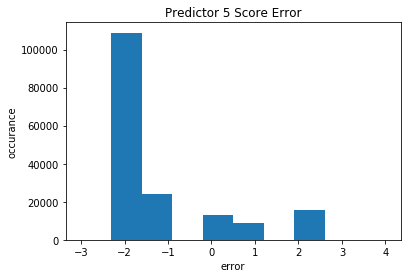
\includegraphics[height=2in, width=2.5in]{predictor_5_error_3}
\caption{Predictor 5 with Default Score set to Middle Score}
\end{figure}

On the other hand, for the train data mean, although there was a up-going trend for MSE, there was a lower degree of increase.
The higher shingle length resulted a less matching chance to the refined database and thus the prediction was more likely to be assigned as train data mean score. This explained the trend of the MSE, which was approaching to the benchmark.

\begin{figure}
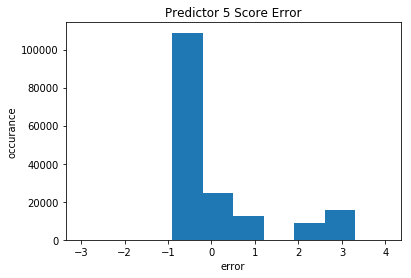
\includegraphics[height=2in, width=2.5in]{predictor_5_error_train_mean}
\caption{Predictor 5 with Default Score set to Train Data Mean}
\end{figure}

The performance could also be compared by examining the spread of error. The above two charts showed the error distributions of 5-shingle prediction of two default scores as an example. From the difference in MSE, the 5-shingle would provide the most obvious divergence in spread.\\
In the first chart, the majority of the error were at two extremes: "-2" and "+2; whilst in the second chart, the crowd was found around "-1". This presented that the Train Data Mean narrowed the error spread and effectively reduced extremes.
The above results concluded that train data mean score should be chosen as the default score.




\subsection{Prediction Method and Refined Database Comparison}

\begin{table}[H]
\caption{Mean Squared Error Comparison using Train Data Mean as Default Score}
	\begin{tabular}{ccc}
			\toprule
				\multirow{2}{*}{Prediction Method} &
				\multicolumn{2}{c}{Refined Database}\\
				\cline{2-3}
				& \texttt{Top-100} &  \texttt{Top-300} \\
				%Method & testing \\
			\midrule
				Train Data Mean & 1.717 & 1.717 \\
				\hline
				1-shingle & 1.596 & 1.592\\
				2-shingle & 1.595 & 1.531\\
				3-shingle & 1.667 & 1.626\\
				4-shingle & 1.704 & 1.701\\
				5-shingle & 1.710 & 1.709\\
				\hline
				Regression & 1.369 & 1.273\\

			\bottomrule
		\end{tabular}

\end{table}

Suppose the train data mean was the default score, the performance of k-shingle method varied. The 1- and 2-shingle outperformed over the five k-shingle method, in which the latter one was slightly better. The reduction in MSE was amplified when using "top-300". Although the match percentage of 2-shingle was much lower than 1-shingle, the prediction turned out to be more accurate. This implied that the 2-shingle offered a more precise indication. In other words, a sentiment expressed more clearly by phrases than words.
However, it applied to 2-shingle only and was another situation for 3-shingle to 5-shingle. When the match percentage further went downwards, the prediction capability tumbled accordingly. \\

\begin{table}[H]

\caption{Regression Coefficient with Train Data Mean as Default Score}
	\begin{tabular}{ccc}
			\toprule
				Regression Coefficient & \texttt{Top-100} &  \texttt{Top-300} \\
			\midrule
				 $\beta_0$ & -8.636 & -13.446\\
				 $\beta_1$ & 1.842 & 3.055\\
				 $\beta_2$ & 0.441 & 0.423\\
				 $\beta_3$ & 0.362 & 0.380\\
				 $\beta_4$ & 0.227 & 0.204\\
				 $\beta_5$ & 0.258 & 0.239\\
				

			\bottomrule
		\end{tabular}

\end{table}

\begin{figure}
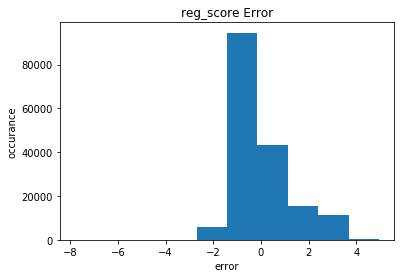
\includegraphics[height=2in, width=2.5in]{reg_error_train_mean_top100}
\caption{"Top-100" Regression Method Error Spread}
\end{figure}

\begin{figure}
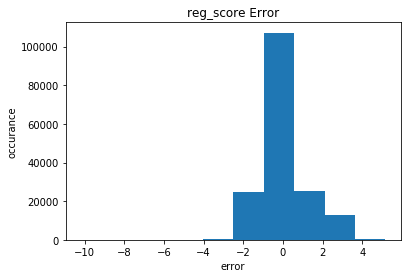
\includegraphics[height=2in, width=2.5in]{reg_error_train_mean_top300}
\caption{"Top-300" Regression Method Error Spread}
\end{figure}


Regression Method provided the least MSE and was superior to k-shingle method. Even though in the worst situation, using the middle score as the default score, it still outperformed and surpassed the benchmark. On one side, this method considered more information, namely all k-shingles; on the other side, it smoothed out the k-shingle predictions and achieved a diminished MSE.\\

Furthermore, in terms of error spread,  Regression Method resulted a bell shape of error distribution. The one from "top-100"  was skewed to the right; while the one of "top-300"  was a bell shape with center at 0.

Comparing "top-100" with "top-300", the larger database always produced lower MSE across all approaches. However, the improvement was noticeable in 2-shingle method and Regression Method. In 2-shingle, the reason was that the match percentage of it was about 13\% higher than the smaller set. In Regression Method, due to the better performance in all k-shingle method, there was a further enhancement in prediction.


\section{Conclusion}

In this project, a several approaches were discovered to predict the sentiment of a paragraph sized text. First, the 2-shingle was the most representative among the 5 shingles. Next, the train data mean should be chosen as the default score. Concerning prediction methods, Regression Method was the best performer; whereas 2-shingle method came out on top of k-shingle method. Finally, a larger refined database provided a lower error.

The prediction methodology could be applied to different aspects of text, such as movie reviews. There was no assumption on the score or sentiment for words at first, unlike using AFINN words rating[1], where it assumed sentiment score for words in advance. In our approach, not only single word, but also phrases or k-shingles were took into consideration. This allowed us to capture the most related wordings or even jargon of the specific topic.

The stopword list was introduced to reduce the size of text and thus the amount of shingles, so as to facilitate the computation. Nevertheless, this resulted not every meaningful phrases were preserved from the stopword list, like, "on the other hand" became "hand", despite the fact that, "hand" was enough to represent it. If one desired to maintain these kind of phrases, they could be excepted during the stopword removal step, or even the step could be skipped. Given that the reviews were in paragraph long, not an article, it would be still acceptable to include all the stopwords. The reason was that the shingle database was constructed by MapRedure or by distributed processing, but the refined database might have to be further reviewed.

Further discussing the size of refined database, it depended on application. For instance, if it applied to streaming data, a smaller refined database would be desirable when the run-time was taken into consideration. In addition, the above result showed that the "top-100" already exceeded the benchmark and there was a trade-off between accuracy and efficiency in facing huge workload. The approach of refined database could also be fine-tuned. For example, it was unnecessary to have same amount of collection in each k-shingle and there could be more 2-shingles.

Linear Regression was introduced to aggregate multi-shingle information. Other regression methods could also be applied, for example, Multiple Linear Regression with higher order variables and Logistic Regression [3].  Taking all 5-shingle prediction scores into account was one of the methods. Other methods such as SVM [4] could also be explored as long as the computation complexity was efficient.


\section{Future Idea}
In this section, we will be exploring some of the idea that can further improve our system.
\subsection{Filtering}
Abuse comments and inconsistent comments to rating will affect the popularity of a product dramatically. For example, many short comments written to lesser the popularity on purpose or a review could be rated with score one but the comment is praising the product. Since our system is able to predict score based on comments by user. We can use the predicted score to filter out abuse comments or ask the reviewer if they make any mistake for inconsistent comments. 

Moreover, filtering can be further improved since the Amazon review now include a indicator showing if the user who left the review did purchase the product or not. If a comment did not get verified of purchasing the product, maybe this comment can be filter out and not include in training the regression model.

\subsection{Streaming Model}
As velocity is one of the important principle of Big Data, this system can be further enhanced to incorporates new comments every minutes. The idea behind is that when a new comment is inserted by a user for a particular product, the system will predict the score based on the comment and see if the predicted result is close to the real rating by the user or not. If not, using regression again to update the coefficient of the equation. This part is also related to the previous filtering part, as we want to filter out abuse comments and inconsistent comments so that when other users read the rating and comment, these comments can truly represent the product.

\begin{thebibliography}{1}
\bibitem{paper2}
	F. {\AA}. Nielsen, 
	{\em AFINN},
	Informatics and Mathematical Modelling, Technical University of Denmark,
	\url{http://www2.imm.dtu.dk/pubdb/p.php?6010},
	Mar 2011.
\bibitem{url}
	{\em List of English Stop Words},
	\url{http://xpo6.com/list-of-english-stop-words/},
	14 Apr 2009.

%[3] 
%Regression reference book
%https://www.amazon.com/Applied-Linear-Regression-Models-Student/dp/0073014664
%
%[4]
%https://dl.acm.org/citation.cfm?id=1246423
%
%[5]
%Amazon Fine Food Reviews
%https://www.kaggle.com/snap/amazon-fine-food-reviews
%




\end{thebibliography}


%\bibliographystyle{ACM-Reference-Format}
%\bibliography{sample-bibliography} 

\end{document}
